%%% user_manual.tex --- 

%% Author: XX.YY@IDEALX.com
%% Version: $Id$

\def\RCS$#1: #2 ${\expandafter\def\csname RCS#1\endcsname{#2}}
\RCS$Revision$
\RCS$Date$

\documentclass{IDXDOC-en}
\usepackage{idx-shortcuts}

% --------------------------------------------
% Title 
% --------------------------------------------
\doctitle{IDX-Tsunami User's manual}

\addauthor{Nicolas}{Niclausse}{nicolas.niclausse@IDEALX.com}

\doccopyright{IDEALX S.A.S.}
\docversion{\RCSRevision}
\docreldate{\RCSDate}
\docref{XXX}

\begin{document}
\maketitle
\Abstract{IDX-Tsunami user's manual}
\newpage
\tableofcontents

\section{Introduction}

\subsection{What is IDX-Tsunami ?}

IDX-tsunami is a distributed load testing tool. It is
protocol-independent and can currently be used to stress HTTP, SOAP
and Jabber servers.



\subsection{What is Erlang and why is it important for IDX-Tsunami ?}

\par IDX-Tsunami main strength is its ability to simulate a huge
number a simultaneous user from a single CPU. When used on cluster
you can generate a really impressive load on a server with a modest
cluster, easy to set-up and to maintain.

\par IDX-Tsunami is developed in Erlang and this is where the power
of IDX-Tsunami relies.

\par Erlang is a \emph{concurrency-oriented} programming language.
Tsunami is based on the Erlang OTP (Open Transaction Platform) and
inherits several characteristics from Erlang: 

\begin{itemize}
\item \emph{Performance}: Erlang has been made to support hundred thousands
of lightweight processus in a single virtual machine. 
\item \emph{Scalability}: Erlang development environnement is naturally
distributed, promoting the idea of processus location transparence. 
\item \emph{Fault-tolerance}:Erlang has been built to develop robust,
fault-tolerant systems. As such, wrong answer sent from the server
to IDX-Tsunami does not make the whole running benchmark crash. 
\end{itemize}

More informations on Erlang on \url{http://www.erlang.org} and
\url{http://www.erlang-projects.org/}


\subsection{IDX-Tsunami background}

History:
\begin{itemize}
\item IDX-Tsunami is being developped since 2001 
\item It is an industrial implementation of a \emph{stochastic model}
for real users simulation. User events distribution is based on a
Poisson Process. More information on this topic in:

Z. Liu, N. Niclausse, et C. Jalpa-Villanueva.  \strong{Traffic Model
  and Performance Evaluation of Web Servers}. \emph{Performance Evaluation,
Volume 46, Issue 2-3, October 2001}.

\item This model has already been tested in the INRIA \emph{WAGON}
  research prototype (Web trAffic GeneratOr and beNchmark). WAGON is
  used in the \url{http://www.vthd.org/} project (Very High Broadband
  IP/WDM test platform for new generation Internet applications).

\end{itemize}

IDX-Tsunami has been used for very high load tests:
 
\begin{itemize}
\item \emph{Jabber} protocol: 10 000 simultaneous users. Tsunami were
running on a 3-computers cluster (CPU 800Mhz) 
\item \emph{HTTP and HTTPS} protocol: 12 000 simultaneous users. IDX-Tsunami
were running on a 4-computers cluster. The tested platform reached
3 000 requests per second. 
\end{itemize}

IDX-Tsunami has been used  at: 

\begin{itemize}
\item \emph{DGI} (Direction G�n�rale des imp�ts): French finance ministry 
\item \emph{Cap Gemini Ernst \& Young}
\item \emph{IFP} (Institut Fran�ais du P�trole): French Research Organization
for Petroleum 
\item \emph{LibertySurf}
\end{itemize}

\section{Features}

\subsection{IDX-Tsunami main features}

\begin{itemize}
\item \emph{High Performance}: IDX-Tsunami can simulate a huge number
of simultaneous users par physical computer: It can simulates up to
10000 users on a single CPU. Traditionnal injection tools can hardly
go further than 200 users. 
\item \emph{Distributed}: the load can be distributed on a cluster of
client machines 
\item \emph{Multi-Protocols} using a plugin system: HTTP (both standard
web traffic and SOAP) and Jabber are currently supported. LDAP and
SMTP are on the TODO list. 
\item \emph{SSL} support 
\item \emph{Several IP addresses} can be used on a single machine using
the underlying OS IP Aliasing 
\item \emph{OS monitoring} (CPU, memory and network trafic) using Erlang
agents on remote servers or \emph{SNMP}
\item \emph{XML configuration system}
\item \emph{Mixed behaviours}: several sessions can be used to simulate
differents type of users during the same benchmark. You can define
the proportion of the various behaviours in the benchmark scenario. 
\item \emph{Stochastic processes}: in order to generate a realistic trafic,
user thinktimes and the arrival rate can be randomize using a probability
distribution (exponential currently) 
\end{itemize}

\subsection{HTTP related features}

\par 


\begin{itemize}
\item HTTP/1.0 and HTTP/1.1 support 
\item GET and POST requests 
\item Cookies: Automatic cookies management 
\item \verb|'|GET If-modified since\verb|'| type of request 
\item WWW-authentication Basic 
\item Proxy mode to record sessions using a Web browser 
\item SOAP support using the HTTP mode (the SOAPAction HTTP header is handled). 
\end{itemize}

\subsection{Jabber related features}

\begin{itemize}
\item Authentication, presence and register messages 
\item Chat messages to online or offline users 
\item Roster set and get requests 
\item Global users\verb|'| synchronisation can be set on specific actions 
\end{itemize}

\subsection{Complete reports set}

\par Mesures and statistics produced by Tsunami are extremely featurefull.
They are all represented as a graphic. Tsumami produces statistics
regarding: 

\begin{itemize}
\item \emph{Performance}: response time, connexion time, decomposition
of the user scenario based on request grouping instruction, requests
per second 
\item \emph{Errors}: Statistics on page return code to trace errors 
\item \emph{Target server behaviour}: An Erlang agent can gather information
from the target server(s). Tsunami produce graphs for CPU and memory
consumption and network traffic. SNMP is also supported. 
\end{itemize}
\par Note that IDX-Tsunami take care of the synchronisation process
by itself. Gathered statistics are �synchronized�.

\par It is possible to generate graphs during the benchmark as statistics
are gathered in real-time.


\section{Installation}

This package has only be tested on Linux. It should work on Erlang
supported platforms (Solaris, *BSD,  Win32 and MacOS-X).

\subsection{Dependencies}
\begin{itemize}
\item Erlang/OTP R9C-0 (\url{http://www.erlang.org/download.html})
\item xmerl-0.19 (\url{http://sowap.sourceforge.net/download.html}). A debian
    binary package is provided at
    \url{http://tsunami.idealx.org/dist/}
  \item extended regexp module (used for dynamic variables):
    gregexp.erl available at
    \url{http://www.cellicium.com/erlang/contribs/} . The module is
    included in the source and binary distribution of IDX-Tsunami. It
    is released under the EPL Licence.
   \item  gnuplot and perl5 (optional; for graphical output with
    analyse_msg.pl script).  The Template Toolkit is used for HTML
    reports (see \url{http://template-toolkit.org/})
  \item  for distributed tests, you need an ssh access to remote machines
    without passwd (use a RSA/DSA key without passphrase or ssh-agent)
\end{itemize}
\subsection{Compilation}

\begin{Verbatim}
./configure (this will detect your erlang installation path)
 make
 make install
\end{Verbatim}
\subsection{Configuration}

The main configuration file is \file{~/.idx-tsunami/idx-tsunami.xml} (
there is a sample file
\file{/usr/share/doc/idx-tsunami/examples/idx-tsunami.xml}).

Log files are saved in \file{~/.idx-tsunami/log/} . A new subdirectory
is created for each test using the current date as name
(\file{~/.idx-tsunami/log/20040217-09:40} for ex.)

\section{HTTP benchmark approach}

\begin{enumerate}
\item Record scenario: \command{idx-tsunami start\_recorder}
\item Edit / organize scenario 
\item Write small code for dynamic parts if needed and place dynamic mark-up
in the scenario 
\item Test and adjust scenario to have a nice progression of the load. This
is highly dependent of the application and of the size of the target
cluster. Calculate the normal duration of the scenario and use the
interarrival time between users and the duration of the phase to estimate
the number of simultaneous users for each given phase. 
\item Launch benchmark with your first application parameters set-up:
  \command{idx-tsunami start}
\item wait for the end of the test or stop by by hand with \command{idx-tsunami stop}
\item Analyse results, change parameters and relaunch another benchmark 
\end{enumerate}

\section{Understanding idx-tsunami.xml configuration file}

\subsection{File structure}

 Scenarii are enclosed into idx-tsunami tags:

 \begin{Verbatim}
<?xml version="1.0"?>
<!DOCTYPE idx-tsunami SYSTEM "idx-tsunami-1.0.dtd" [] >
<idx-tsunami loglevel="info" dumptraffic="false">
...
</idx-tsunami>
 \end{Verbatim}


\subsection{Clients and server}

 Scenarii start with a clients (Tsunami cluster) and server definition:

\begin{Verbatim}
  <clients>
     <client host="louxor" weight="1" maxusers="500">
         <ip value="10.9.195.12"></ip>
         <ip value="10.9.195.13"></ip>
     </client>
     <client host="memphis" weight="3" maxusers="250" cpu="2">
         <ip value="10.9.195.14"></ip>
     </client>
  </clients>

  <server host="10.9.195.1" port="8080" type="tcp"></server>
 \end{Verbatim}

 
 Several virtual IP can be used to simulate more machines. This is
 very useful when a load-balancer use the client\verb|'|s IP to
 distribute the traffic amoung a cluster of servers. 
 
 In this example, a second machine is used in the Tsunami cluster,
 with a higher weight, and 2 cpus. Two Erlang virtual machines will be
 used to take advantage of the number of CPU.
 
 The server is the entry point into the cluster (Only one server
 should be defined).


\subsection{Monitoring}

\par Scenarii can contain optional monitoring informations. For example,
here is a cluster monitoring definition based on Erlang agents, for
a cluster of 6 computers:

\begin{Verbatim}
  <monitoring>
    <monitor host="geronimo" type="erlang"></monitor>
    <monitor host="bigfoot-1" type="erlang"></monitor>
    <monitor host="bigfoot-2" type="erlang"></monitor>
    <monitor host="f14-1" type="erlang"></monitor>
    <monitor host="f14-2" type="erlang"></monitor>
    <monitor host="db" type="erlang"></monitor>
  </monitoring>
\end{Verbatim}

The type keyword snmp can replace the erlang keyword, if SNMP monitoring
is prefered. They can be mixed. erlang is the default value for monitoring.

\par Note: For Erlang monitoring, monitored computers need to be
accessible through the network. SSH needs to be configured to allow
connection without password on.


\subsection{Defining the load progression}

\par The load progression is set-up by defining several arrival phases:

\begin{Verbatim}
  <arrivalphase phase="1" duration="10" unit="minute">
    <users interarrival="2" unit="second"> </users>
  </arrivalphase>

  <arrivalphase phase="2" duration="10" unit="minute">
    <users interarrival="1" unit="second"> </users>
  </arrivalphase>

  <arrivalphase phase="3" duration="10" unit="minute">
    <users interarrival="0.1" unit="second"> </users>
  </arrivalphase>
\end{Verbatim}

\subsection{Default values}

\par Default values can be set-up globally: thinktime between requests
in the scenario and ssl cipher algorithms. These values overrides
those set in session configuration tags.
\begin{Verbatim}
  <default name="thinktime" value="3" random="false"/>
  <default name="ssl_ciphers" 
           value="EXP1024-RC4-SHA,EDH-RSA-DES-CBC3-SHA"/>
\end{Verbatim}


Default values for specific protocols can be defined. Here is an
example of default values for Jabber:

\begin{Verbatim}
  <default type="ts_jabber" name="global_number" value="5" />
  <default type="ts_jabber" name="userid_max" value="100" />
  <default type="ts_jabber" name="domain" value="jabber.org" />
  <default type="ts_jabber" name="username" value="glop" />
  <default type="ts_jabber" name="passwd" value="glop" />
\end{Verbatim}

\subsection{Sessions}

Sessions define the content of the scenario itself. They describe
the requests to execute.

\begin{Verbatim}
  <session name="http-example" popularity="70" type="ts_http">

    <request> <http url="/" method="GET" version="1.1">
                    </http> </request>
    <request> <http url="/images/logo.gif"
               method="GET" version="1.1" 
               if_modified_since="Fri, 14 Nov 2003 02:43:31 GMT">
              </http></request>

    <thinktime value="20" random="true"></thinktime>

    <transaction name="index_request">
     <request><http url="/index.en.html"
                          method="GET" version="1.1" >
              </http> </request>
     <request><http url="/images/header.gif"
                          method="GET" version="1.1">
              </http> </request>
    </transaction>

    <thinktime value="60" random="true"></thinktime>
    <request>
      <http url="/" method="POST" version="1.1"
               contents="bla=blu">
      </http> </request>
    <request>
       <http url="/bla" method="GET" version="1.1"
             contents="bla=blu&name=glop">
       <www_authenticate userid="Aladdin"
                         passwd="open sesame"/></http>
    </request>
  </session>

  <session name="backoffice" popularity="30" ...>
  ... </session>
\end{Verbatim}

The popularity is the frequency of this type of session. This is used
to decided which session a new user will execute. The sum of all
session\verb|'|s popularity must be 100. 

This example show several features of the HTTP protocol support in
Tsunami: GET and POST request, basic authentication, transaction for
statistics definition, ...

\par Here is an example of a session definition for the Jabber protocol:
\begin{Verbatim}
 <session popularity="70" name="jabber-example" type="ts_jabber">

    <request> <jabber type="connect" ack="no_ack" />
                    </request>
    <thinktime value="2"></thinktime>
    <transaction name="authenticate">
      <request> <jabber type="authenticate" ack="local">
                      </jabber> </request>
    </transaction>

    <request> <jabber type="presence" ack="no_ack"/> 
                </request>
    <thinktime value="2"></thinktime>

    <request> <jabber type="register" ack="no_ack" 
                     id="new"></jabber> </request>

    <transaction name="roster">
      <request><jabber type="iq:roster:set" ack="no_ack" 
                              destination="offline" />
      </request>
      <request><jabber type="presence:roster" ack="no_ack"
                              destination="previous"/>
      </request>
      <request><jabber type="iq:roster:set" ack="no_ack"
                             destination="online"/>
      </request>
      <request><jabber type="iq:roster:get" ack="no_ack">
                  </jabber> </request>
    </transaction>
    <thinktime value="2"></thinktime>

    <request> <jabber type="chat" ack="no_ack"
                           size="56"/></request>
    <thinktime value="30"></thinktime>

    <transaction name="global_msg">
    <request> <jabber type="chat" ack="global" size="56"
                           destination="random"/></request>
    </transaction>

    <thinktime value="30"></thinktime>

    <transaction name="online">
    <request> <jabber type="chat" ack="no_ack" size="16"
                          destination="online"/></request>
    </transaction>
    <thinktime value="30"></thinktime>

    <transaction name="offline">
      <request> <jabber type="chat" ack="no_ack" size="56"
                             destination="offline"/><request>
    </transaction>

    <thinktime value="30"></thinktime>

    <transaction name="close">
      <request> <jabber type="close" ack="local">
                </jabber></request>
    </transaction>

  </session>

  <session popularity="30" name="jabber-example2" ...>
  ... </session>  
\end{Verbatim}

\subsection{Dynamic substitutions}

 Dynamic substitution are mark-up placed in element of the scenario.
For HTTP, this mark-up can be placed in basic authentication (www\_authenticate
tag: userid and passwd attributes), URL (to change GET parameter)
and POST content.

Those mark-up are of the form \userinput{\%\%Module:Function\%\%}.
Substitutions are executed on a request-by-request basis, only if the
request tag has the attribute \userinput{subst=\verb|"|true\verb|"|}.

When a substitution is asked, the substitution mark-up is replaced by
the result of the call to the Erlang function:
\userinput{Module:Function(Pid)}.

Here is an example of use of substitution in a Tsunami scenario:

\begin{Verbatim}
<session name="rec20040316-08:47" popularity="100" type="ts_http">
 <request subst="true">
  <http url="/echo?symbol=%%symbol:new%%" method="GET">
  </http></request>
</session>
\end{Verbatim}

 Here is the Erlang code of the module used for dynamic substitution:

\begin{Verbatim}
-module(symbol).
-export([new/1]).

new(Pid) ->
    case random:uniform(3) of
        1 -> "IBM";
        2 -> "MSFT";
        3 -> "RHAT"
    end.
\end{Verbatim}

As you can this, writing scenario with dynamic substitution is trivial.

If you want to set unique id, you can use the function
\varname{ts_user_server:get_unique_id}.
\begin{Verbatim}
<session name="rec20040316-08:47" popularity="100" type="ts_http">
 <request subst="true">
  <http url="/echo?id=%%ts_user_server:get_unique_id%%" method="GET">
  </http></request>
</session>
\end{Verbatim}

\subsection{Dynamic variables}

In some cases, you may want to use a value given by the server in a
response later in the session, and this value is \strong{dynamically
generated} by the server for each user. For this, you can use
\userinput{<dyn_variable>} in the scenario

Let's take an exemple with HTTP. You can easily grab a value in a HTML
form like:
\begin{Verbatim}
<form action="go.cgi" method="POST">
<hidden name="random_num" value="42"></form>
</form>
\end{Verbatim}

\begin{Verbatim}
 <request>
   <http url="/testtsunami.html" method="GET" version="1.0"></http>
   <dyn_variable name="random_num" ></dyn_variable>
 </request>
\end{Verbatim}

Now \varname{random_num} will be set to 42 for the user session. It's
value will be replace in all mark-up of the form
\userinput{\%\%_random_num\%\%} if and only if the request tag has the
attribute \userinput{subst=\verb|"|true\verb|"|}, like:

\begin{Verbatim}
    <request subst="true">
      <http url='/go.cgi' version='1.0' 
      contents='username=nic&amp;random_num=%%_random_num%%&amp;op=login' 
      content_type='application/x-www-form-urlencoded' method='POST'>
      </http>
    </request>
\end{Verbatim}
  
If the dynamic value is not a form variable, you can set a regexp by
hand, for example to get the title of a HTML page:
\begin{Verbatim}
    <request>
      <http url="/testtsunami.html" method="GET" version="1.0"></http>
      <dyn_variable name="mytitlevar" 
                    regexp="&lt;title&gt;\(.*\)&lt;/title&gt;"/>
    </request>
\end{Verbatim}


\section{Statistics and reports}

Availables stats:
\begin{itemize}
\item  request (response time for each request)
\item  page (response time for each set of requests)
\item  connect (duration of the connection)
\item  reconnect (number of reconnection)
\item  size (size of responses)
\item  session (duration of a user's session)
\item  users (number of simultaneous users)
\item  custom transactions
\end{itemize}

HTTP specific stats:
\begin{itemize}
\item counter for each response status (200, 404, etc.)
\end{itemize}


\subsection{Generating the report}

cd to the log directory of your test (say
\file{~/.idx-tsunami/log/20040325-16:33/}) and use the script
\command{analyse\_msg.pl}:

\begin{Verbatim}
/usr/lib/idx-tsunami/bin/analyse_msg.pl --stats idx-tsunami.log  --html --extra  --plot  
\end{Verbatim}

\subsection{Tsunami summary}
\begin{figure}[htb]
  \begin{center}
    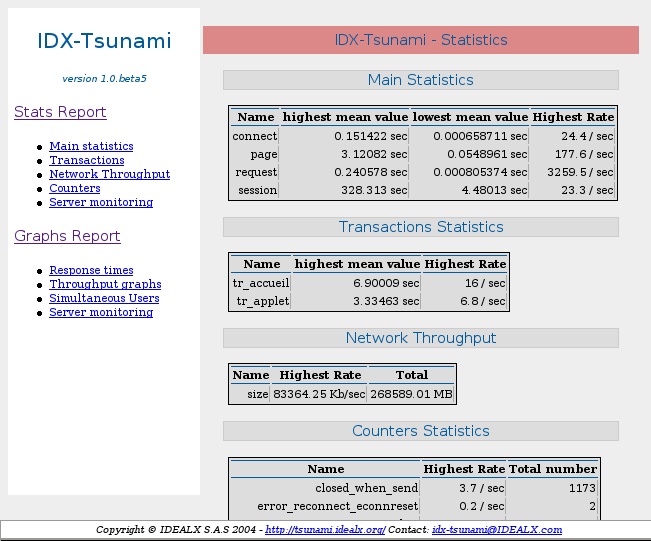
\includegraphics[width=0.6\linewidth]{tsunami-report}
    \end{center}
      \caption{Report}
    \label{fig:report}
\end{figure}

\subsection{Graphical overview}


\begin{figure}[htb]
  \begin{center}
    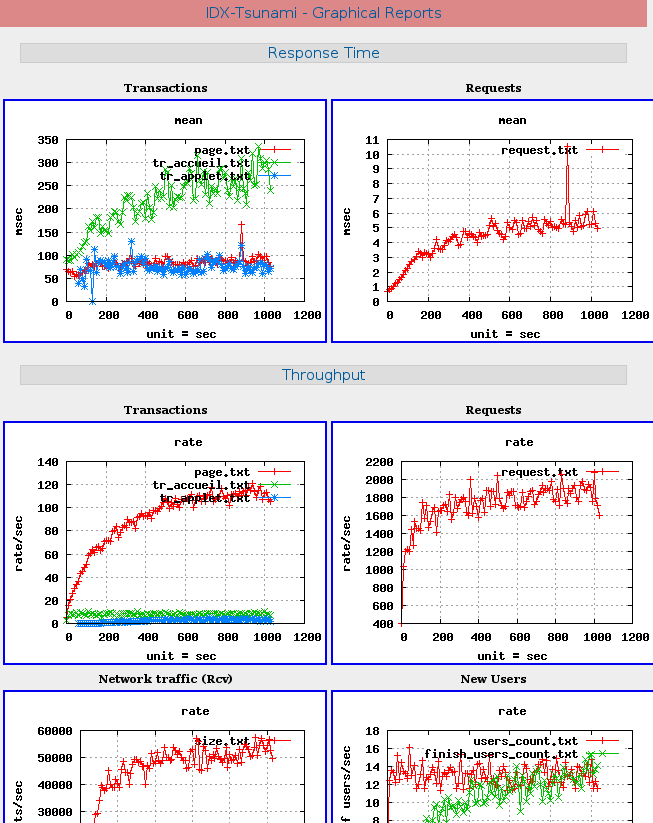
\includegraphics[width=0.6\linewidth]{tsunami-graph}
    \end{center}
      \caption{Graphical output}
    \label{fig:graph}
\end{figure}

\section{Conclusion}

IDX-Tsunami has several advantages over other injection tools: 


\begin{itemize}
\item \emph{Outstanding performance} and \emph{distributed benchmark}
\item \emph{Ease of use}: The hard work is already done for all supported
protocol. No need to write complex scripts. Dynamic scenarii only
requires small trivial piece of code.
% Tsunami scenarii realisation is mostly based on 
\item \emph{Multi-protocol support}: IDX-Tsunami is for example one of
the only tool to benchmark SOAP applications 
\item \emph{Monitoring} of the target cluster to analyse the behaviour
and find bottlenecks. For exemple, I did use it to analyse cluster
symmetry (is the load properly balanced ?) and to determine the best
combination of machines on the three cluster tiers (Web engine, EJB
engine and database) 
\end{itemize}

\subsection{Roadmap}

FIXME

\subsection{References}

\begin{itemize}
\item IDX-Tsunami home page: \url{http://tsunami.idealx.org/}
\item IDX-Tsunami description (French)\footnote{\url{http://www.erlang-projects.org/Members/mremond/events/dossier_de_presentat/block_10766817551485/file}}
\item Erlang web site \url{http://www.erlang.org/}
\item Erlang programmation, Micka�l R�mond, Editions Eyrolles, 2003
  \footnote{\url{http://www.editions-eyrolles.com/php.accueil/Ouvrages/ouvrage.php3?ouv_ean13=9782212110791}}
\item Making reliable system in presence of software errors, Doctoral Thesis,
Joe Armstrong, Stockholm, 2003 \footnote{\url{http://www.sics.se/~joe/thesis/armstrong_thesis_2003.pdf}}
\end{itemize}

\subsection{Acknowledgements}

The first version of this document is based on a talk given by Mickael
R�mond\footnote{\url{mickael.remond@erlang-fr.org}} during an Object
Web benchmarking workshop in April 2004 (more info at
\url{http://jmob.objectweb.org/}).


\begin{appendix}

\section{Frequently Asked Questions}

\subsection{IDX-tsunami crash when I start it }

Does your erlang system has ssl support enabled ?

to test it:
\begin{Verbatim}
  > erl
  Eshell V5.2  (abort with ^G)
  1> ssl:start()
  you should see 'ok' 
\end{Verbatim}

\subsection{IDX-tsunami still crash  when I start it}
First look at the log file
\file{~/.idx-tsunami/log/XXX/tsunami_controller@yourhostname'} to see
if there is a problem. 

Remember that you can validate your configuration file using the
provided DTD !

If you see nothing wrong, you can compile \program{idx-tsunami} with full
debugging: set OPTIONS to \userinput{+debug_info -DDEBUG} in the Makefile, and
don't forget to set the loglevel to "debug" in the XML file.

To start the debugger or see what happen, start IDX-Tsunami with the
\userinput{debug} argument instead of \userinput{start}. You will have
an erlang shell on the \varname{tsunami_controller} node. Use
\command{toolbar:start().} to launch the graphical tools provided by
Erlang.
\subsection{What is the format of the stats file idx-tsunami.log ?}

\begin{Verbatim}
# stats: dump at 1045817668
 stats: reconnect 1 11
 stats: page_resptime 2 23.9185 1.83948 202.245 22.0790 2 
 stats: size 58269 664029
 stats: response_time 5 3.04958 1.40884 25.6390 1.84204 5 
 stats: 200 2 16
 stats: 404 3 49
 # stats: dump at 1045817678
 stats: reconnect 1 12
 stats: page_resptime 1 56.2450 0.00000e+0 202.245 22.0790 1 
 stats: size 120028 784057
 stats: response_time 1 56.2450 0.00000e+0 56.2450 1.84204 1 
 stats: 200 1 17
 stats: 404 0 49
 ...
\end{Verbatim}

 the format is, for page_resptime, response_time, session:

\texttt{ # stats:'name' count(during the last 10sec), mean, stdvar,
  max, min, count(again, useless)}

 or for HTTP returns code, size, reconnect ...

\texttt{ # stats:'name' count(during the last 10sec), totalcount(since the beginning)}

\subsection{How can i specify the number of concurrent users ?}

You can't. But it's on purpose: the load generated by IDX-Tsunami is
dependent on the arrival time between new clients. Indeed, once a
client has finished his session in \program{idx-tsunami}, it stops. So the
number of concurrent users is a function of the arrival rate and the
mean session duration.

For example, if your web site has $1000$ visits/hour, the arrival rate
is $1000/3600 = 0.2778$ visits/second. If you want to simulate the same
load, set the inter-arrival time is to $1/0.27778 = 3.6 sec$ (\texttt{<users
interarrival="3.6" unit="second">} in the \varname{arrivalphase} node in the
XML config file).

\subsection{SNMP monitoring doesn't work ?!}

There is a small bug in the \file{snmp_mgr} module (R9C release). You have to
apply this patch to make it work.


\begin{Verbatim}
--- lib/snmp-3.4/src/snmp_mgr.erl.orig  2004-03-22 15:21:59.000000000 +0100
+++ lib/snmp-3.4/src/snmp_mgr.erl       2004-03-22 15:23:46.000000000 +0100
@@ -296,6 +296,10 @@
     end;
 is_options_ok([{recbuf,Sz}|Opts]) when 0 < Sz, Sz =< 65535 ->
     is_options_ok(Opts);
+is_options_ok([{receive_type, msg}|Opts]) ->
+    is_options_ok(Opts);
+is_options_ok([{receive_type, pdu}|Opts]) ->
+    is_options_ok(Opts);
 is_options_ok([InvOpt|_]) ->
     {error,{invalid_option,InvOpt}};
 is_options_ok([]) -> true.
\end{Verbatim}

\end{appendix}

\end{document}


%%% for AucTex/Emacs : 
%%% Local Variables: 
%%% eval:(setenv "TEXINPUTS" ":.:../../common/styles:../commmon/images:../common/figures:")
%%% mode: latex
%%% End: 
